\section{Обзор литературы}
\label{sec:domain}

\subsection{Обзор существующих технологий}
\label{sub:domain:technologies_review}

Современные методы обработки изображений делятся на две основные категории: программная и аппаратная обработка.

Программная обработка производится на базе центрального проессора(CPU) и отличается высокой эффективностью
при использовании последовательных алгоритмов \cite{asano_dip_comp}. В задачах с высоким Data Level Parallelism по обработке гомогенных данных
центральный процессор значительно проигрывает более специализированным решениям,
из-за малого количества SIMD блоков для параллельной обработки данных \cite{axell_cpu_simd}.

Комбинация программных и аппаратных подходов лежит в основе обработки изображений на графическом процессоре (GPU).
Связка графического процессора и SDK для его программирования образует GPGPU (General-Purpose computing for GPU).
GPGPU основна на прицнипе SIMT, основанный на разделении задачи на несколько подзадач того же типа, но меньшего размера,
решаемые каждым потоком GPU по отдельности.
Такой подход является удачной комбинацией скорости разработки программы и специализации графического процессора
на параллельной обработке данных \cite{patterson_hennessy}.

Однако есть и существенные ограничения.
Латентность при обработке изображений на GPU слабодетерменирована, что усложняет использование GPGPU
в системах реального времени \cite{maceina_gpu_real_time}.
Отсутствует выбор периферийного интерфейса -- на момент написания,
графический процессоры подключаются исключительно по PCIe(PCI express), сильно ограничивая перечень устройств.
Соотношение производительности на ватт затрудняет применение во встраиваемых системах с автономным питанием \cite{fowers_gpu_power_consumption}.

ASIC(Application-Specific Integrated Circuit), как наиболее специализированное на конкретной задаче решение, выполняет обработку за минимально возможное время
и с минимальным энергопотреблением \cite{amara_asic_low_power}. Разработка специализированной интегральной схемы связана
с существенными затратами на проектирование --- окупаемость наступает лишь при выпуске партиями в несколько сотен тысяч единиц,
исключая возможность применения технологии малыми и средними предприятиями \cite{smith_asic_economy}.

Применение FPGA(Field Programmable Gate Array) достичь баланса между производительностью и конфигурируемостью конечного решения.
По сравнению с ASIC единовременные затраты на проектирование на несколько порядков ниже,
что идеально подходит для прототипирования и мелкосерийного производства \cite{zuchowski_asic_vs_fpga_cost}.
В отличие от GPU малое энергопотребление и небольшие размеры решений на FPGA прекрасно подходят
для встраиваемых систем \cite{berten_gpu_fpga_comparison}.
Последовательные алгоритмы, непригодные для реализации на GPU, могут выполняться
на интегрированом CPU или soft core процессоре, заметно упрощая передачу данных
между последовательным и параллельным вычислителем, решая подобную задачу
для связки GPU и CPU \cite{russo_softcore_fpga_vs_gpu}.

Таким образом, оптимальной технологией для реализации аппаратной системы обработки видеопотока,
с поддержкой модульности и достаточного быстродействия является технология FPGA.


\subsection{Технология FPGA}
\label{sub:domain:fpga}

FPGA(Field Programmable Gate Array) --- программируемые пользователем вентильные матрицы,
представляет собой наиболее общий и современный класс программируемой логики.
Основные области применения FPGA:
\begin{itemize}
  \item разработка блоков и систем на стадии их прототипирования, даже при дальнейшей их реализации на другой технологической базе;
  \item реализация конечных продуктов небольшого тиража, тем самым уменьшая затраты на проектирование до возможного минимума.
\end{itemize}

Данные характеристики обеспечиваются удачной комбинацией общих и узкоспециализированных средств
в пределах одной микросхемы. Внутренняя область FPGA содержит множество идентичных конфигурируемых логических блоков(КЛБ),
которые соединены трассами межсоединений. По периметру микросхемы расположены блоки ввода-вывода(БВВ).

Базовая структура FPGA приведена на рисунке~\ref{fig:domain:fpga:fpga_architecture}

\begin{figure}[ht]
  \centering
  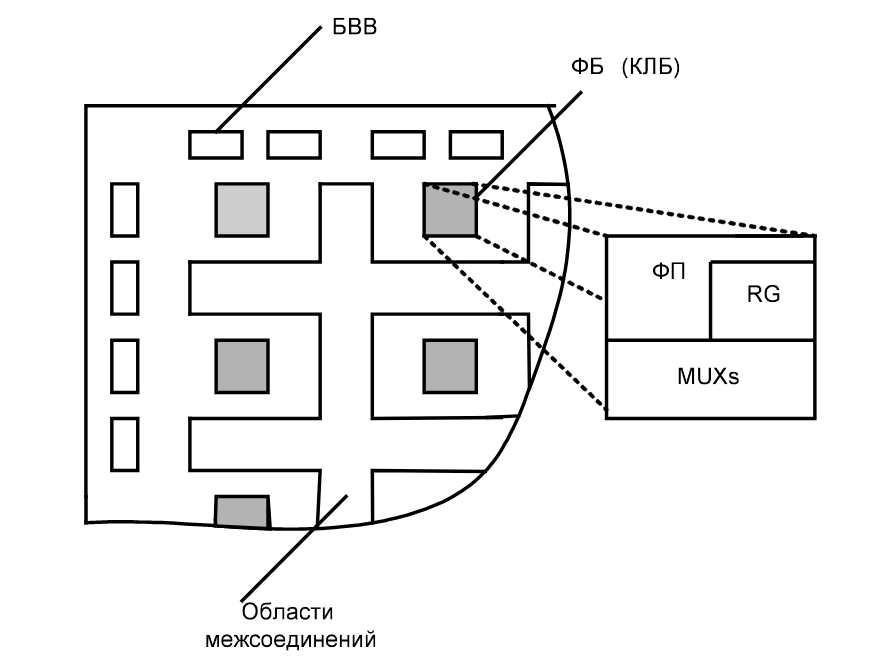
\includegraphics[scale=0.35]{ugrymov_fpga_artchitecture.png}
  \caption{ Фрагмент базовой архитектуры FPGA \cite{ugrymov_digital_circuit_engineering} }
  \label{fig:domain:fpga:fpga_architecture}
\end{figure}

Конфигурируемые логические блоки состоят из:
\begin{itemize}
  \item некоторого количества элементов выполняющих логические преобразования;
  \item набора мультиплексоров для перенаправления выходных сигналов логических преобразователей;
  \item триггеров для хранения значений сигналов.
\end{itemize}

Схема современного КЛБ на примере семейства Spartan компании Xilinx представлена на рисунке~\ref{fig:domain:fpga:clb}

\begin{figure}[ht]
  \centering
  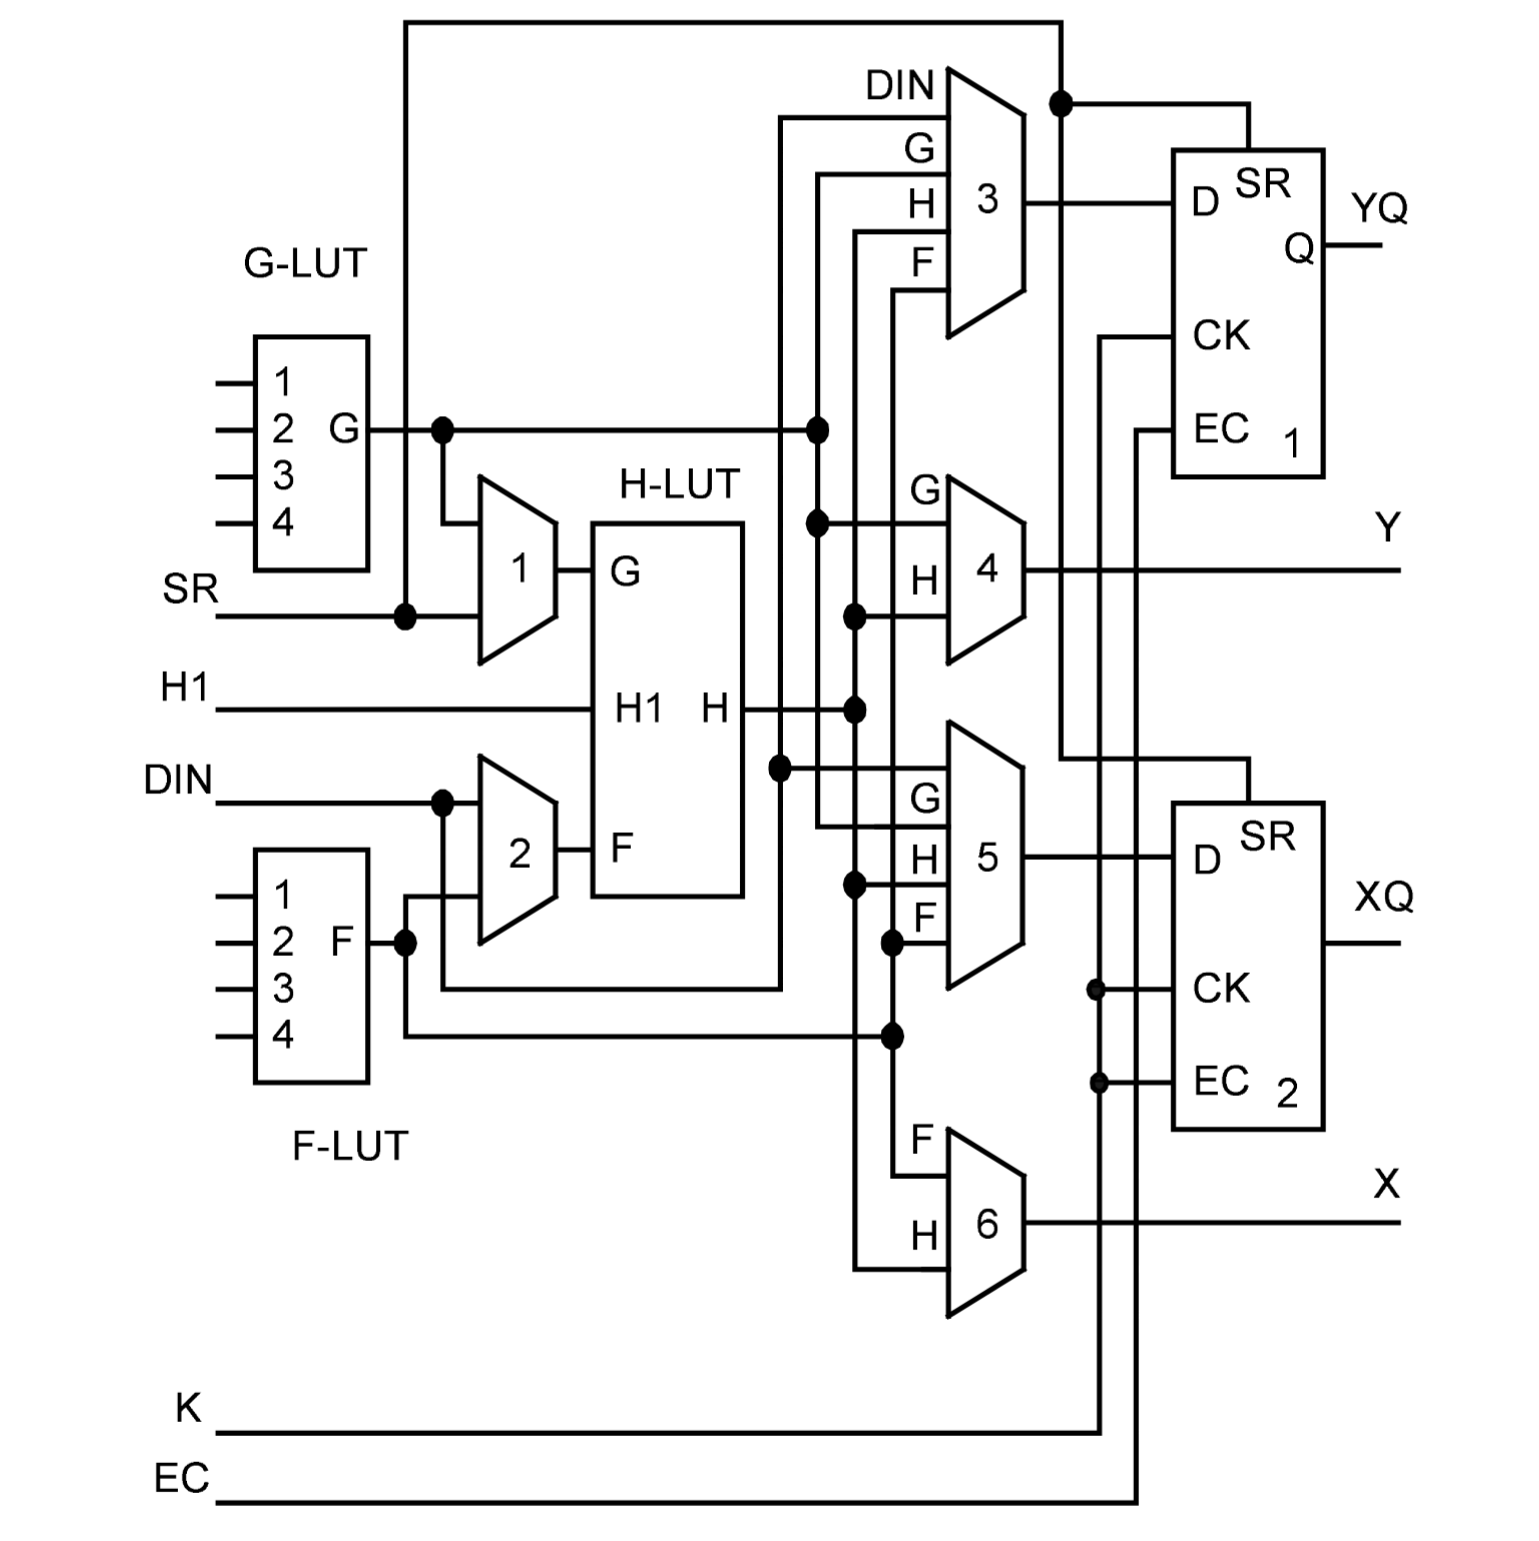
\includegraphics[scale=0.25]{ugrymov_fpga_clb.png}
  \caption{ Логический блок семейсва Spartan }
  \label{fig:domain:fpga:clb}
\end{figure}

Системы межсоединений проектируются в широком диапазоне технологических и архитектурных решений.
Основная цель при построении эффективной системы коммутации --- обеспечение максимальной коммутируемости блоков
при минимальном количестве элементов связи с предсказуемыми задержками сигналов. Обозрение данной тематики задача достаточно нетривиальная,
стоит лишь отметить, что предсказуемость задержек это ключевой фактор в выборе микросхемы для проектирования системы реального времени.

С каждым выводом микросхемы ассоциируется свой блок ввода-вывода, который может настраиваться как вход, выход или двунаправленный вывод.
Упрощенная схема блока В/В представлена на рисунке~\ref{fig:domain:fpga:io}

\begin{figure}[ht]
  \centering
  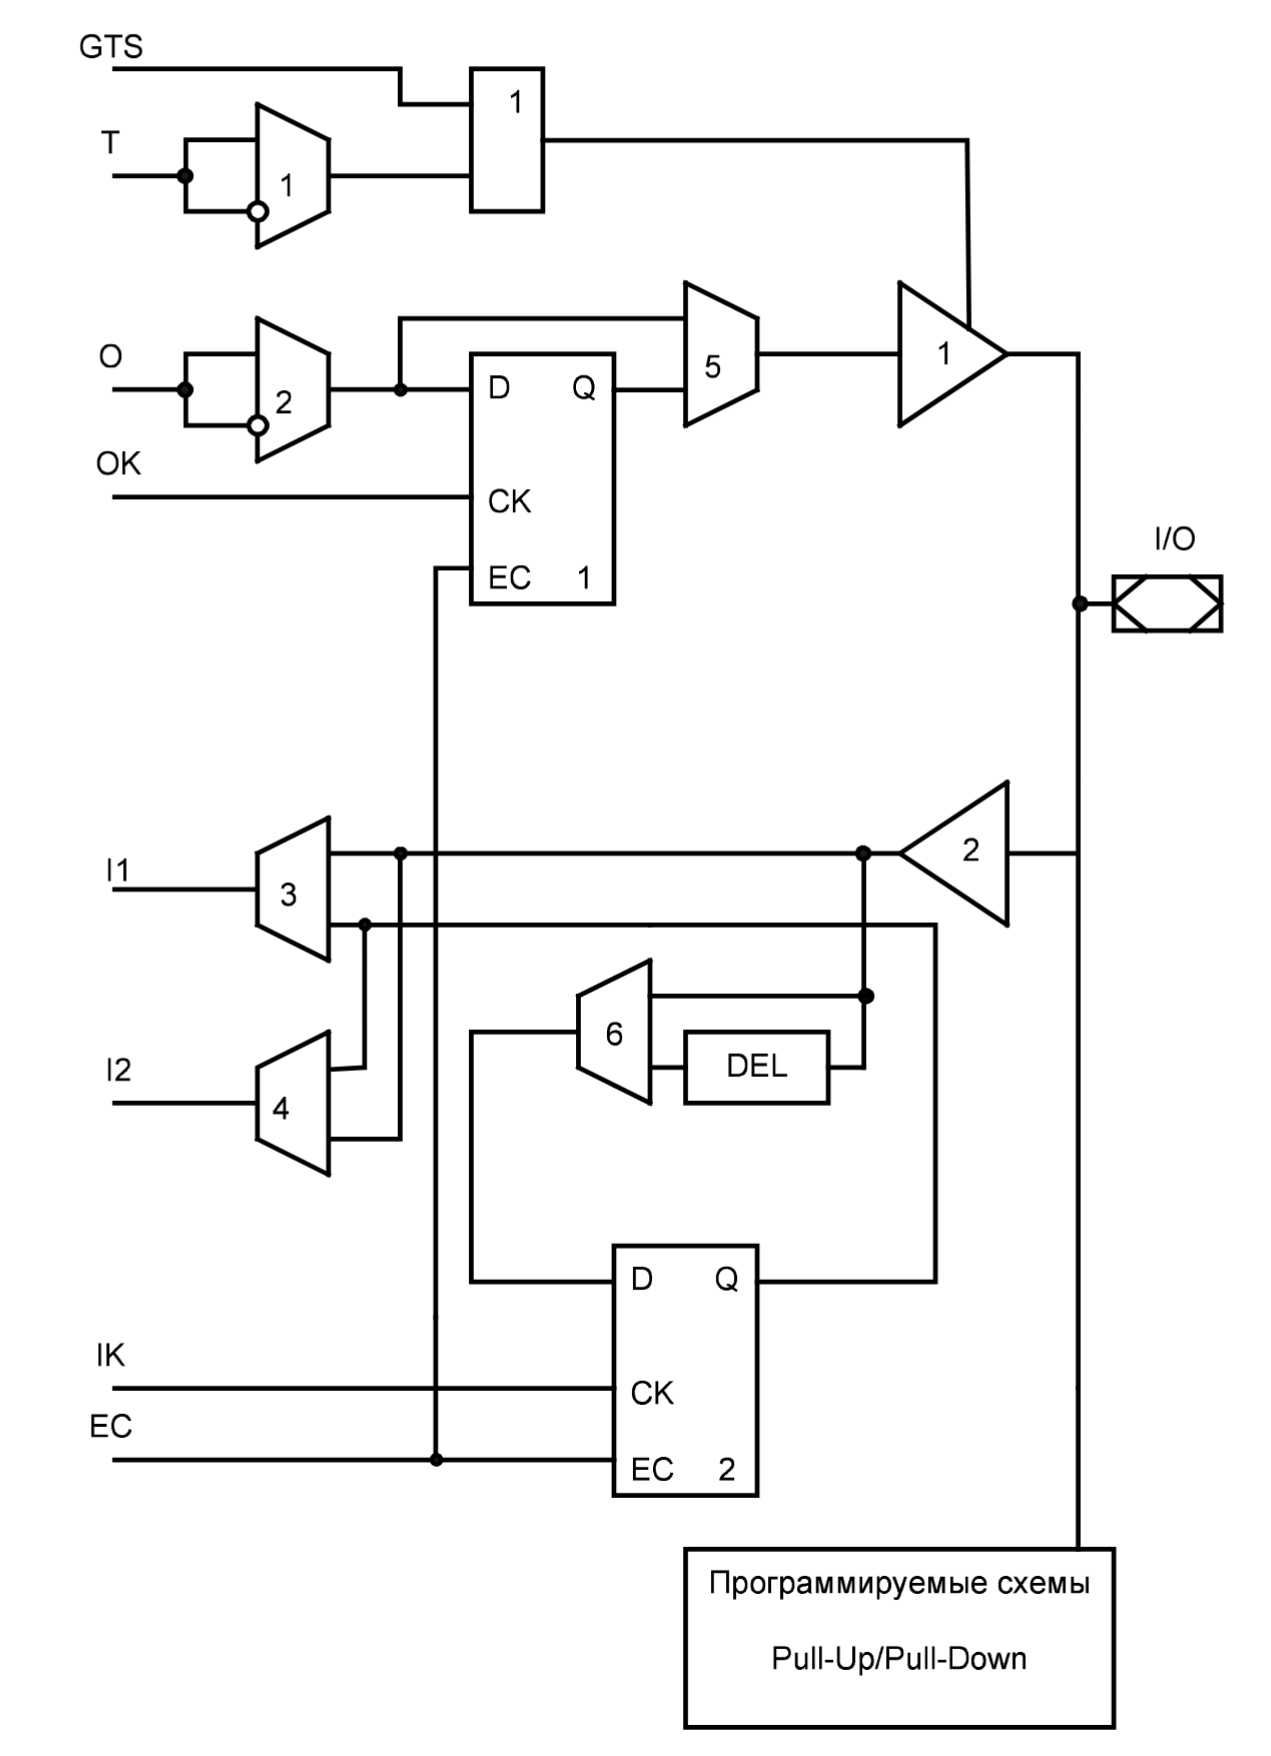
\includegraphics[scale=0.25]{ugrymov_fpga_io.png}
  \caption{ Пример схемы блока ввода-вывода FPGA }
  \label{fig:domain:fpga:io}
\end{figure}

Блок разделен на две части для работы как на вход, так и на выход. Основной интерес представляют буферы с тремя состояниями
1 и 2. Они имеют програмимруемые уровни сигналов(КМОП или ТТЛ), что заметно упрощает подключение пользовательских периферийных устройств
напрямую к микросхеме без поключения внешнего преобразователя уровня.

Основными игроками на рынке микросхем FPGA являются Xilinx и Altera. Они производят чипы применимые как в военной и космической сферах,
так и для потребительских нужд. Микросхемы широко варьируются по количеству логических блоков, размеру
статической памяти, количеству блоков ввода-вывода и поддержкой специфических блоков.

Однако для проектирования и отладки системы важен выбор не только микросхемы,
но и отладочной платы с необходимым набором периферии. Подробное сравнение отладочных
плат с микросхемами последнего поколения от различных производителей показывает, что
платы с микросхемами Xilinx наиболее разнообразы и представлены в более широком ценовом диапазоне,
чем платы Altera \cite{fpga_boards_comparison}.
Вследствие чего сделан выбор применения микросхем Xilinx в дипломном проекте.

\subsection{Сравнение cемейств микросхем Xilinx}
\label{sub:domain:fpga_comparison}

Компания Xilix является технологическим лидером на рынке производства микросхем FPGA.
На данный момент наиболее актуальная линейка микросхем --- Xilinx 7 series.
Продукты данной линейки покрывают всевозможные требования к микросхеме: от низкого энергопотребления, малого размера, низкой цены до
поддержки высокоскоростных интерфейсов и большого количества логических и DSP(Digital Signal Processing) блоков.

Седьмое поколение микросхем Xilinx делится на 4 основные категории:
\begin{itemize}
  \item Spartan-7: для недорогих и маломощных систем, требующих высокую производительность ввода-вывода.
    Имеет наименьшую площадь посадочного места во всей линейке;
  \item Artix-7: оптимизирован для маломощных приложений с требованиями по высокой пропуской способности логических и DSP блоков.
    Обладает наиболее высоким параметром производительности на ватт;
  \item Kintex-7: микросхема с лучшим соотношением цены к производительности,
\end{itemize}

% Плюсы fpga конкретно для DIP dark fantasies

% Параллелизм в алгоритмах обработки изображений существует в двух основых формах --- пространственный и временный.
% Реализации данных алгоритмов на FPGA потенциально могут использовать комбинацию двух форм.\cite{downton_dip_architectures}.

% В частости, в задачах обработки изображения, FPGA ценится за возможность применения в системах
% с динамической реконфигрурацией, в которых требуется быстрая смена настроек системы для подстраивания
% под изменяющиеся внешние параметры \cite{burns_fpga_run_time_reconf}.

\subsection{Обзор платы AC701}
\label{sub:domain:ac701}

Плата AC701 от компании Xilinx представляет собой так называемый evaluation board,
содержащую весь возможный набор периферийных устройств подключемых к микропроцессору.
Среди них особый интерес представляют:
\begin{itemize}
  \item микросхема XC7A200T-2FBG676C семейства Artix-7;
  \item 1GB DDR3 SODIMM;
  \item Fixed 200MHz LVDS осциллятор;
  \item программируемый осциллятор I2C;
  \item FMC(FPGA Mezzanine Card);
  \item шина I2C разведённая ко всей программируемой на плате периферии;
  \item контроллер и коннектор HDMI.
\end{itemize}

Стурктурная схема платы представлена на рисунке~\ref{fig:domain:ac701:block_design}

\begin{figure}[ht]
  \centering
  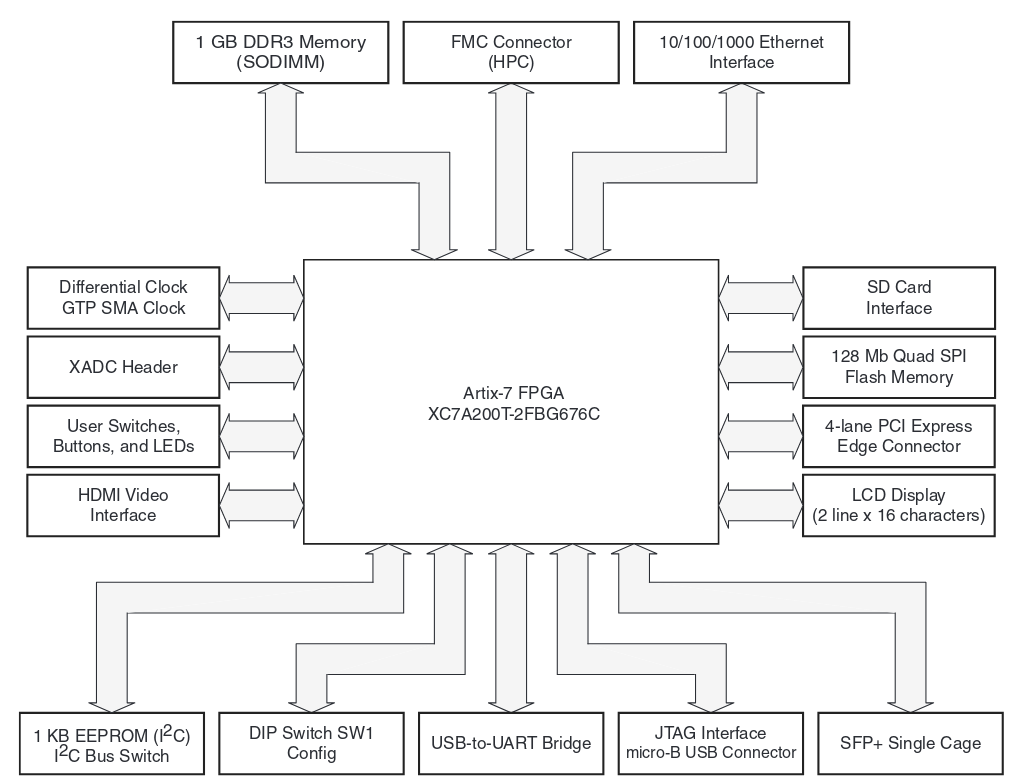
\includegraphics[scale=0.4]{ac701_block_design.png}
  \caption{ Блок схема платы AC701 }
  \label{fig:domain:ac701:block_design}
\end{figure}


\subsection{Обзор видеоинтерфейсов}
\label{sub:domain:videointerfaces}



\subsection{Обзор камер}
\label{sub:domain:camera}


\subsection{Принцип минимальной длинны описания}
\label{sub:domain:mdl_principle}
В данном подразделе рассматривается принцип минимальной длинны описания\footnote{В англоязычной литературе используется термин minimum description length или сокращенно MDL.} (МДО) и его применимость для задания функции оценки качества обучаемой сети.
Данный принцип позволяет среди множества моделей выбрать модель с оптимальным соотношением сложности и соответствием модели наблюдаемым данным.
Т.\,е. данный принцип позволяет выбрать несложную и <<полезную>> модель, устойчивую к проблеме переобучения\footnote{В англоязычной литературе данная проблема называется overfitting и подразумевает, что модель слишком хорошо объясняет данные на которых она обучалась, но из-за этого непригодна для прогнозирования "--- работе на данных ранее не известных.}.
Принцип МДО в своей нестрогой и наиболее общей формулировке гласит: среди множества моделей следует выбрать ту, которая позволяет описать данные наиболее коротко, без потери информации~\cite{Grunwald05atutorial}.
В контексте поиска модели байесовой сети, соответствующей экспериментальным данным, принцип МДО гласит, что нужно выбрать модель, которая минимизирует сумму длин кодирования самой модели и кодирования экспериментальных данных с помощью этой модели~\cite{Lam94learningbayesian}, что выражается формулой:
\begin{equation}
  \label{eq:domain:mdl:description_length}
  l(x^{R}[n]) = \min_{g \in G}\left[ l_{G}(g) + l_{g}(x^{R}[n]) \right] \text{\,,}
\end{equation}
\begin{explanation}
где & $ x^R $ & вектор размерностью $R$, содержащий значения переменных (аттрибутов). Представлен как $ x^R =\newline= (x^{(1)}, x^{(2)}, \dotsc, x^{(R)} ) $, где атрибут $ x^{(j)} $ может принимать $ \alpha_{j} $ значений, $ j = 1,\dotsc,R.$ \\
    & $ n $ & количество случаев в экспериментальных данных;  \\
    & $ x^R[n] $ & набор экспериментальны данных; \\
    & $ G $ & множество моделей; \\
    & $ l_{G}(g) $ & длина описания модели; \\
    & $ l_{g}(x^{R}[n]) $ & длина представления данных $ x^R[n] $ моделью $ g \in G $.
\end{explanation}

Для вычисления длинны кодирования модели и длинны кодирования данных с использованием модели в реализации дипломного проекта использовались результаты, приведенные в работах~\cite{Suzuki93,terentyev_2006}.
Собственно модель вероятностной сети состоит из таблиц условных и безусловных распределений и отношений <<родитель"=потомок>> между вершинами.
Для вычисления длины кодирования модели можно воспользоваться формулой~(\ref{eq:domain:mdl:model_length}):
\begin{equation}
  \label{eq:domain:mdl:model_length}
  l_{G}(g) = \frac{\log{n}}{2} \cdot \sum_{k = 1}^{R} S_k(g) (\alpha_k - 1) \text{\,,}
\end{equation}
\begin{explanation}
где & $ S_k(g) $ & количество возможных назначений переменных"=родителей переменной $X_k$, способ вычисления данного значения отличается у классических сетей и модификации упомянутой в разделе~\ref{sub:domain:bayes_net} на странице~\pageref{page:domain:bayes_mod}.
\end{explanation}

Значение функции $S_k(g)$ для классических байесовых сетей вычисляется по формуле~(\ref{eq:domain:mdl:classic_parent_states}), для модификации упомянутой в разделе~\ref{sub:domain:bayes_net} на странице~\pageref{page:domain:bayes_mod} "--- по формуле~(\ref{eq:domain:mdl:mod_parent_states}):
\begin{align}
  \label{eq:domain:mdl:classic_parent_states}
  S_k(g) &= \prod_{j \in \pi_k}\alpha_j \text{\,,} \\
  \label{eq:domain:mdl:mod_parent_states}
  S_k(g) &= \sum_{j \in \pi_k}\alpha_j \text{\,.}
\end{align}

Длинна представления данных $ l_{g}(x^{R}[n]) $ вычисляется как эмпирическая энтропия $ n $ экспериментальных наблюдений $ x^{R}[n] $ при заданной модели $ g $.
Эмпирическая энтропия может быть вычислена по формуле~(\ref{eq:domain:mdl:data_entrophy}):
\begin{equation}
  \label{eq:domain:mdl:data_entrophy}
  \mathcal{H}(x^{R}[n] | g) =
    \sum_{k = 1}^{R}
    \sum_{s = 1}^{S_{k}(g)}
    \sum_{q = 0}^{\alpha_{k + 1} - 1}
    -n[q, s, k, g] \log \frac{n[q, s, k, g]}{n[s, k, g]} \text{\,,}
\end{equation}
\begin{explanation}
где & $ n[s, k, g] $ & количество случаев в экспериментальных данных $ x^R[n] $ в которых переменные"=родители переменной $X_k$ принимают назначение $s$; \\
    & $ n[q, s, k, g] $ & количество случаев в экспериментальных данных $ x^R[n] $ в которых переменные"=родители переменной $X_k$ принимают назначение $s$, а переменная $X_k$ принимает назначение $q$.
\end{explanation}

Таким образом, приведенные выше формулы, могут быть использованы для оценки качества структуры сети и её сложности.
Имея данную оценку можно использовать различные стратегии поиска в пространстве возможных моделей, минимизируя целевую функцию~(\ref{eq:domain:mdl:description_length}).
Более подробно об используемых стратегиях поиска говорится в разделе~\ref{sec:arch_and_mod}.
За доказательствами и более подробными сведениями о применении принципа МДО в построении байесовых сетей можно обратиться к работам~\cite{Lam94learningbayesian,Suzuki93,terentyev_2006,Grunwald05atutorial}.

% MDL (2-3)


\subsection{Оценка структуры сети на основе апостериорной вероятности}
\label{sub:domain:k2_algo}
Существуют подходы, использующие байесов метод для оценки качества полученной структуры и алгоритмы на их базе пытаются максимизировать апостериорную вероятность структуры для данного набора экспериментальны данных.
Один из возможных подходов к оценке качества двух структур приведет в работе~\cite{Cooper1991}.
В программном обеспечении, разработанном в данном дипломном проекте, использовался критерий оценки качества структуры, приведенный в упомянутой выше работе.

Введем некоторые обозначения, в дополнение к тем, которые были введены в подразделе~\ref{sub:domain:mdl_principle}.
Пусть структура вероятностной сети обозначается символом $B_S$, таблицы условных распределений, ассоциированные с сетью, "--- $B_P$.
Две вероятностные сети для данного набора экспериментальных данных можно оценить по отношению~(\ref{eq:domain:k2:nets_ratio}) апостериорных вероятностей:
\begin{equation}
  \label{eq:domain:k2:nets_ratio}
  \frac{P(B_{S_i} | x^R[n])}{P(B_{S_j} | x^R[n])} =
    \frac{ \frac{P(B_{S_i}, x^R[n])}{P(x^R[n])} }
         { \frac{P(B_{S_j}, x^R[n])}{P(x^R[n])} } =
    \frac{ P(B_{S_i}, x^R[n]) }
         { P(B_{S_j}, x^R[n]) } \text{\,.}
\end{equation}

Как видно из приведенной формулы~(\ref{eq:domain:k2:nets_ratio}), научившись вычислять отношение совместных распределений, можно сравнивать апостериорные вероятности структур.
Т.\,к. в разработанном ПО использовались результаты, приведенные в работе~\cite{Cooper1991}, то считаем целесообразным привести в данном подразделе базовые формулы и предположения из вышеупомянутой работы.

Для вычисления $P(B_S, D)$ важно сделать несколько важных предположений:

\begin{itemize}
  \item
  Экспериментальные данные содержат только дискретные случайные величины и все эти случайные величины присутствуют в истинной структуре $B_S$ модели из которой были получены эти экспериментальные данные.
  Из данного предположения следует формула~(\ref{eq:domain:k2:assumption1}):
  \begin{equation}
    \label{eq:domain:k2:assumption1}
    \int_{B_P} P(x^R[n] | B_S, B_P) f(B_P | B_S) P(B_S) dB_p \text{\,,}
  \end{equation}
  \par\hspace{\fivecharsapprox} % абзацный отступ
  \begin{tabular}{@{}ll@{ --- }p{0.74\textwidth}}
  где & $ B_P $ & вектор, содержащий значения условных вероятностей для назначений переменных из структуры $ B_S $; \\
      & $ f $ & условная плотность распределения $B_P$ при условии структуры $B_S$. \\[\parsep]
  \end{tabular}

  \item
  Случаи, зафиксированные в экспериментальных данных, независимы друг от друга, при условии зафиксированной модели, т.\,е. данное предположение подразумевает, что модель, генерирующая экспериментальные данные не меняется.
  Это предположение позволяет упростить формулу~(\ref{eq:domain:k2:assumption1}) и привести её к виду:
  \begin{equation}
    \label{eq:domain:k2:assumption2}
    P(B_S, x^R[n]) =
      P(B_S) \int_{B_P} \left[ \prod_{j = 1}^{n} P(x^R_j | B_S, B_P) \right] f(B_P | B_S) dB_P \text{\,.}
  \end{equation}

  \item
  Экспериментальные данные не должны содержать пропущенных значений для переменных из структуры $B_S$.
  Введем дополнительные обозначения.
  Пусть $x_j^{(i)}$ представляет значение $i$-й переменной в $j$-м случае.
  Пусть $\phi_i$ представляет из себя вектор уникальных назначений переменных"=родителей для $i$-й переменной, т.\,е. вектор уникальных назначений для $ \forall X_k,\ k \in \pi_i$.
  Пусть $\sigma(i, j)$ индексная функция, которая возвращает индекс назначения $\pi_i$ в $j$-ом случае из вектора $\phi_i$.
  Введем обозначение для длинны вектора $q_i = | \phi_i |$.
  Теперь с учетом предположения об отсутствии пропущенных значений можно вычислить вероятность конкретного случая из экспериментальных данных по формуле:
  \begin{equation}
    \label{eq:domain:k2:case_prob}
    P(x^R_j | B_S, B_P) =
      \prod_{i = 1}^{R} = P(X_i = x_j^{(i)} | \phi_i[\sigma(i, j)], B_P) \text{\,.}
  \end{equation}
  Подставляя выражение~(\ref{eq:domain:k2:case_prob}) в формулу~(\ref{eq:domain:k2:assumption2}) получим:
  \begin{align}
    \label{eq:domain:k2:assumption3}
    P(B_S, x^R[n]) =
      P(B_S)
      \int_{B_P}\left[ \prod_{j = 1}^{n}\prod_{i = 1}^{R} P(X_i = x_j^{(i)} | \phi_i[\sigma(i, j)], B_P)  \right] &\times \notag\\
      \times f(B_P | B_S) dB_P \text{\,.}
  \end{align}
  Пусть для выбранных $i$ и $j$ $f(P(x_i | \phi_i[j], B_P))$ обозначает плотность распределения возможных значений $P(x_i | \phi_i[j], B_P)$.
  Необходимо сделать еще одно предположение.

  \item Для $ 1 \le i, i' \le n$, $ 1 \le j \le q_i $, $1 \le j' \le q_i $, если
  $ij \neq i'j'$, то распределение $f(P(x_i | \phi_i[j]))$ не зависимо от распределения $f(P(x_{i'} | \phi_{i'}[{j'}]))$.
  Данное предположение по свой сути полагает, что до того, как были получены экспериментальные данные, все возможные назначения равновероятны.
\end{itemize}

С учетом приведенных выше предположений и теоремы, приведённой и доказанной в работе~\cite{Cooper1991}, можно привести формулу для вычисления $P(B_S, D)$:
\begin{equation}
  \label{eq:domain:k2:model_and_data_prob}
  P(B_S, x^R[n]) =
    P(B_S)
    \prod_{i = 1}^{R}
    \prod_{j = 1}^{q_i}
    \frac{(\alpha_i - 1)!}
         {(n[\phi_i[j], i, B_S] + \alpha_i - 1)!}
    \prod_{k = 1}^{\alpha_i}
      n[v_{ik}, \phi_i[j], i, B_S]! \text{\,,}
\end{equation}
\par
\begin{tabular}{@{}ll@{ --- }p{0.74\textwidth}}
где & $ v_{ik} $ & $k$-е возможное назначение переменной $X_i$. \\[\parsep]
\end{tabular}

Формула~(\ref{eq:domain:k2:model_and_data_prob}) позволяет вычислить значение $P(B_S, x^R[n])$, если известна вероятность $P(B_S)$ и подсчитана оставшаяся часть формулы на основе экспериментальны данных $x^R[n]$.
Но из-за того, что $P(B_S)$ является чаще неизвестной величиной, чем известной, предполагают, что все возможные структуры сети равновероятны и $P(B_S)$ является некой малой константой.
Апостериорную вероятность структуры, при условии данных можно вычислить по формуле:
\begin{equation}
  \label{eq:domain:k2:aposteriori_structure_given_data}
  P(B_S | x^R[n]) =
    \frac{P(B_S, x^R[n])}
         {\sum_{B_S}P(B_S, x^R[n])} \text{\,.}
\end{equation}

Но, как уже упоминалось, множество возможных структур слишком велико, и на практике значение апостериорной вероятности можно вычислить лишь для малых сетей либо приблизительно.
В разделе~\ref{sec:arch_and_mod} будет более подробно рассмотрена модификация оценки апостериорной вероятности~(\ref{eq:domain:k2:model_and_data_prob}), применимая на практике.

%Оценка апостериорных вероятностей (K2) (2-3)

\subsection{Общая структура алгоритмов}
\label{sub:domain:other_algos}
В предыдущих двух подразделах были рассмотрены два подхода к оценке качества структуры сети при известных экспериментальных данных.
Как уже упоминалось ранее, выбор функции оценки сети является лишь одним из компонентов большинства алгоритмов построения структуры сети по данным.
Важной частью алгоритма является также выбор стратегии поиска в пространстве возможных структур.
От выбора стратегии поиска зависит трудоемкость алгоритма, качество найденной сети и, собственно, её структура.
В ПО разработанном в рамках дипломного проекта реализовано несколько различных алгоритмов нахождения структуры на основе оценки апостериорной вероятности из подраздела~\ref{sub:domain:k2_algo} и оценки на основе принципа МДО из подраздела~\ref{sub:domain:mdl_principle}.
Стоит упомянуть, что в разработанном ПО реализованы разные стратегии поиска для разных оценок.
Так алгоритмы использующие оценку МДО могут находить сети произвольной структуры без каких-либо априорных знаний о предметной области.
С другой стороны, для уменьшения пространства возможных решений, алгоритм, использующий оценку апостериорной вероятности, требует априорных знаний об упорядоченности переменных.
В данном конкретном случае, переменные должны быть упорядочены так, что возможные переменные"=родители данной переменной находятся в упорядоченном списке раньше самой переменной.
Во многих других работах накладываются дополнительные ограничения на структуру выводимой сети.
Например, в работе~\cite{Suzuki93} используется оценка МДО, но класс находимых структур ограничен деревьями.
В работе~\cite{Rebane87} приводится алгоритм, ограниченный классом полидеревьев.
% Ограничения других методов построения (упорядоченность нод, ) (2)

\subsection{Обзор существующих программ} % (fold)
\label{sub:domain:existing_programs}
Cуществует множество решений для работы с классическими байесовыми сетями.
Ниже приведены некоторые из задач, которые может выполнять типичный редактор вероятностных сетей:
\begin{itemize}
  \item ручное, автоматическое, полу"=автоматическое построение структуры сети;
  \item оценка параметров условных распределений по данным;
  \item различные алгоритмы статистического вывода суждений в сетях;
  \item генерация экспериментальных данных по готовой сети;
\end{itemize}

Приняв во внимание тему дипломного проекта, наибольший интерес в существуем ПО будет представлять функциональность автоматического вывода структуры сети по данным.
Ниже рассматриваются некоторые из программ для работы с байесовыми сетями.

\subsubsection{SAMIAM }(\url{http://reasoning.cs.ucla.edu/samiam})
Бесплатный кросс"=платформенный редактор байесовых сетей, написанный на Java.
Имеет богатую функциональность по ручному созданию сетей.
Поддерживает множество различных алгоритмов вывода статистических суждений и позволяет делать различные типы запросов к сети.
Позволяет генерировать экспериментальные данные, соответствующие готовой сети.
Но функциональность, обеспечивающая автоматический вывод структуры сети по данным, отсутствует.

\subsubsection{Netica }(\url{http://www.norsys.com/netica.html})
Коммерческое программное обеспечение.
Версия программы с ограниченной функциональностью свободно доступна на сайте фирмы Norsys.
Netica "--- мощная, удобная в работе программа для работы с графовыми вероятностными моделями.
Она имеет интуитивный и приятный интерфейс пользователя для просмотра и редактирования топологии сети.
Соотношения между переменными могут быть заданы, как индивидуальные вероятности, в форме уравнений, или путем автоматического обучения из файлов данных (которые могут содержать пропуски), но, к сожалению, в бесплатном варианте программы данная функциональность недоступна и возможности сравнить с разработанной в дипломном проекте реализацией нет.
Созданные сети могут быть использованы независимо, и как фрагменты более крупных моделей, формируя тем самым библиотеку модулей~\cite{terehov_2003}.

\subsubsection{GeNIe }
\label{sub:domain:existing_programs:genie}
(\url{http://genie.sis.pitt.edu/})
Бесплатное кросс"=платформенное приложение и библиотека для работы с вероятностными графовыми моделями, написанная на \cpp{}.
Предоставляется функциональность ручного и автоматического создания сетей, а также реализуются алгоритмы вывода статистических суждений.
Программа реализует несколько алгоритмов вывода структуры сети по данным, целесообразно привести здесь одно небольшое сравнение с разработанным ПО, т.\,к. функциональности приложений пересекаются.
Более подробное сравнение разработанного ПО с существующим будет произведено в разделе~\ref{sec:arch_and_mod}.
Уместно рассмотреть хорошо изученную сеть Asia\footnote{\url{http://www.bnlearn.com/bnrepository/\#asia}}.
Экспериментальные данные, содержащие \num{1000} случаев и имеющие распределение задаваемое сетью, были сгенерированы с помощью одной из вышеперечисленных программ.
К этим экспериментальным данным были применены три различных алгоритма вывода структуры, реализованные в GeNIe.
Выведенные структуры приведены на рисунке~\ref{fig:domain:programs:genie_infered_structrures}.
Для сравнения, структуры, выведенные одним из алгоритмов из разработанной библиотеки на том же наборе данных, и истинная сеть Asia приведены на рисунке~\ref{fig:domain:programs:our_impl_plus_asia}.
Как видно, алгоритм из разработанной библиотеки не нашел одну связь, в отличие от алгоритмов реализованных в GeNIe, которые допустили больше ошибок в структуре.

\begin{figure}[ht]
\centering
  \begin{subfigure}[b]{0.51\textwidth}
    \centering
    \includegraphics[scale=0.5]{asia_genie_1000_bayesian_search.pdf}
    \caption{}
  \end{subfigure}
  \begin{subfigure}[b]{0.48\textwidth}
    \centering
    \includegraphics[scale=0.5]{asia_genie_1000_k2.pdf}
    \caption{}
  \end{subfigure}
  \begin{subfigure}[b]{0.9\textwidth}
    \centering
    \includegraphics[scale=0.5]{asia_genie_1000_pc.pdf}
    \caption{}
  \end{subfigure}
  \caption{ Структуры, выведенные по данным с помощью GeNIe: а "--- алгоритм Bayesian Search;
            б "--- алгоритм K2;
            в "--- алгоритм PC;}
  \label{fig:domain:programs:genie_infered_structrures}
\end{figure}


\begin{figure}[ht]
\centering
  \begin{subfigure}[b]{0.49\textwidth}
    \centering
    \includegraphics[scale=0.45]{asia-learned-by-terent-random-1000.pdf}
    \caption{}
  \end{subfigure}
  \begin{subfigure}[b]{0.48\textwidth}
    \centering
    \includegraphics[scale=0.45]{asia_reference_net.pdf}
    \caption{}
  \end{subfigure}

  \caption{ Выведенная из данных и оригинальная сеть Asia: а "--- алгоритм из разработанной библиотеки, использующий оценку МДО;
            б "--- истинная сеть Asia}
  \label{fig:domain:programs:our_impl_plus_asia}
\end{figure}